Comme nous l'avons détaillé dans le \autoref{chap:04}, la phase de
décomposition est subdivisible en trois étapes (décomposition de
l'ensemble des indices de localisation, des \emph{objets de référence
  indéfinis}, et des \emph{relations de localisation}), dont seule la
dernière nécessite le développement d'une méthode spécifique. En
effet, les étapes de décomposition de ensemble des \emph{indices de
  localisation} et des \emph{objets de référence indéfinis} ne
qu'expliciter un découpage présent dès la saisie. Ces deux opérations
ne nécessitent donc pas l'apport de connaissances supplémentaires,
contrairement à la décomposition des \emph{relations de localisation.}

En effet, les \emph{principes de décomposition} et de
\texttt{intégration contexte métier} s'opposent en partie. Si la
décomposition permet de faciliter la \emph{spatialisation} des
\emph{indices de localisation} en permettant de manipuler des concepts
précis et en minimisant les redondances, elle implique également de
travailler à l'aide de \emph{relations de localisation} (atomiques)
\emph{ad hoc,} qui ne sont pas conçues pour être faciles à manipuler
par l'utilisateur et encore moins pour être proche des \emph{relations
  de localisations} qu'elles décomposent. Il est donc difficilement
envisageable de demander à l'utilisateur de saisir directement les
\emph{relations de localisation} décomposées (\ie les \emph{relations
  de localisation atomiques}). C'est pourquoi nous proposons
d'automatiser cette étape.

Pour ce faire il est nécessaire de définir au préalable la manière
dont les différentes \emph{relations de localisation} spatialisables
se décomposent (cf. présentation du \emph{principe de modélisation
  explicite des connaissances}, \autoref{chap:04}). Nous avons choisi
de formaliser ces décomposition au sein d'une ontologie, créée pour
l'occasion. Pour permettre la décomposition des \emph{relations de
  localisation} cette dernière doit contenir, a minima, trois types
d'informations :
%
\begin{enumerate*}[label=(\alph*)]
\item \emph{les relations de localisation} à décomposer,
\item les \emph{relations de localisation atomiques} qui les
  décomposent et
\item les \emph{relations de décomposition} formalisant la
  décomposition d'une \emph{relation de localisation} en plusieurs
  \emph{relations de localisations atomiques}
  (\autoref{fig:onto_min_struct}).
\end{enumerate*}
%
L'ensemble des \emph{relations de localisation} définies dans
l'ontologie forme un vocabulaire contrôlé, permettant à l'utilisateur
de saisir les \emph{indices de localisation}. La décomposition de ces
relations ne lui est pas connue. Le travail de décomposition ne
consiste alors qu'a identifier la \emph{relation de localisation}
utilisée et à identifier les \emph{relations de localisation
  atomiques} qui la décomposent à l'aide des \emph{relations de
  décomposition} définies dans l'ontologie.

\begin{figure}
  \centering
  \usetikzlibrary{patterns}
\usetikzlibrary{fadings}
\usetikzlibrary{external}
\usetikzlibrary{calc}
\usetikzlibrary{positioning}
\usepgfplotslibrary{colormaps}
\usetikzlibrary{arrows}
\usetikzlibrary{matrix}

\usetikzlibrary{trees}


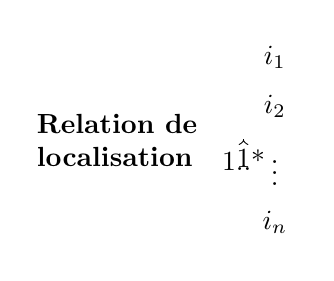
\begin{tikzpicture}
  \tikzset{
    acc/.style={decorate,decoration={brace,raise=0cm,amplitude=.1cm}},
    accm/.style={acc,decoration={mirror}},
    acc3/.style={acc,decoration={amplitude=.2cm}},
    acc3m/.style={acc3,decoration={mirror}}
  }
  
%% Matrices
\node[font=\bfseries, baseline, text width=2.5cm] (I) at (0,0) {Relation de localisation};

\matrix [matrix of math nodes,row sep=0.1cm,column sep=0.1cm,
anchor=west, nodes={anchor=base, baseline}] (is) at (I.east)
{i_1\\i_2\\\vdots{}\\i_n\\};

\draw[->, black] (I.east) -- (is.west) node[pos=0,below] {1} node[pos=1,below]{1..*};

\end{tikzpicture} 
  \caption{Éléments nécessaires pour permettre de décomposer une
    \emph{relation de localisation} ($rl_i$) en un ensemble de
    \emph{relations de localisation atomiques} ($rla_i$).}
  \label{fig:onto_min_struct}
\end{figure}

Comme nous l'expliquions lors de la présentation de la phase de
décomposition, chacune des étapes de cette phase consiste à créer un
nouvel \emph{indice de localisation.} Conformément au \emph{principe
  de modélisation autonome,} chaque \emph{indice de localisation}
traité peut être décomposé de manière indépendante.

Comme le montre la \autoref{fig:onto_min_struct}, plusieurs
configurations de décompositions sont envisageables. La première
d'entre-elles, la plus courante, est la décomposition d'une
\emph{relation de localisation} en plusieurs \emph{relations de
  localisation atomiques} (\eg \(rk_1\) et \(rl_3\),
cf. \autoref{fig:onto_min_struct}). Ces dernières peuvent partager une
\emph{relation de localisation atomique} (\eg \(rk_2\) et \(rl_3\)
dont la décomposition contient \(rla_3\)), ce qui est souhaité par le
\emph{principe de décomposition.} Dans certaines configurations (\eg
\(rl_2\)), on ne peut pas identifier de décomposition satisfaisante
pour une \emph{relation de localisation.} La \emph{relation de
  localisation} n'est alors que l'alias d'une \emph{relation de
  localisation atomique.} Dans ce cas il n'est pas nécessaire de
définir (contrairement a ce qui a été fait pour l'exemple de la
\autoref{fig:onto_min_struct}), une \emph{relation de localisation} et
une \emph{relation de localisation atomique,} on peut simplement
définir la seconde et la présenter à l'utilisateur comme une
\emph{relation de localisation non atomique.}


%%% Local Variables:
%%% mode: latex
%%% TeX-master: "../../../../main"
%%% End:
